\chapter{Infrastructure}

The infrastructure of the hosted GitLab service in our OpenStack platform consists of:
\begin{itemize}
    \item n Runners (at the moment 1) in a separate 'gitlabrunners' network, which is not public accessible
    \item One public facing server which hosts GitLab itself in the 'provider' network,
          the Runners need to access this server via the 'gitlabrunners' network
\end{itemize}

\section{Networks}

The 'gitlabrunners' network has a network address of '10.0.0.0/24' and a gateway IP of '10.0.0.254'.
The DHCP range is defined as '10.0.0.100-10.0.0.200'.\\

The Runners need to access the internet, for installation of packages/updates, but also for getting data to be used in the CI process (e.g. getting Docker images) 
That is the reason why also a router is added for this network.

\section{GitLab}

\subsection{Machine and network configuration}

A machine with flavor 'm1.large' with 'Debian-11' as base image is used for the machine of the self-hosted GitLab instance.
This is due to CPU, memory and software requirements of GitLab and Docker.\\

A floating IP is leased and used for the 'provider' network.
Due to the availability of the domain 'gruber.info', an A-record for the \ac{fqdn} 'gitlabtest.gruber.info' is used (\ref{fig:a_record}) and an https certificate is generated for that \ac{fqdn} via Let´s encrypt (\ref{fig:lets_encrypt}).
This certificate is used to prevent errors in the https communication.
\begin{figure}[H]
	\centering
	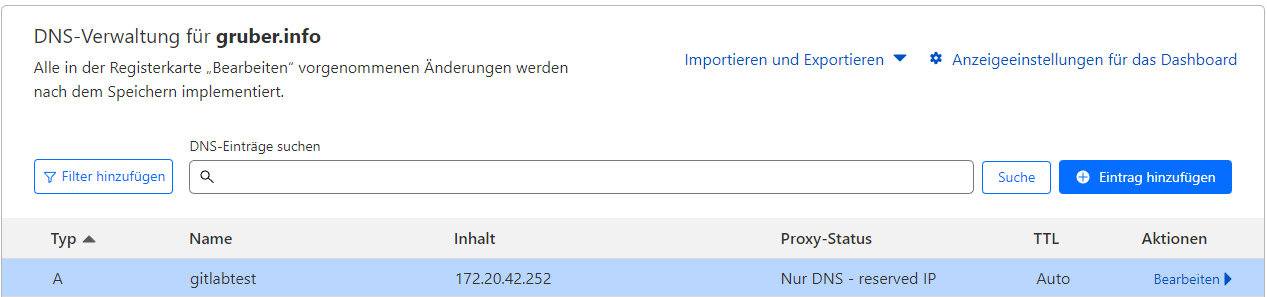
\includegraphics[width=14cm]{images/a-record.png}
	\caption{'gitlabtest.gruber.info' as A-record}
	\label{fig:a_record}
\end{figure}

\begin{figure}[H]
	\centering
	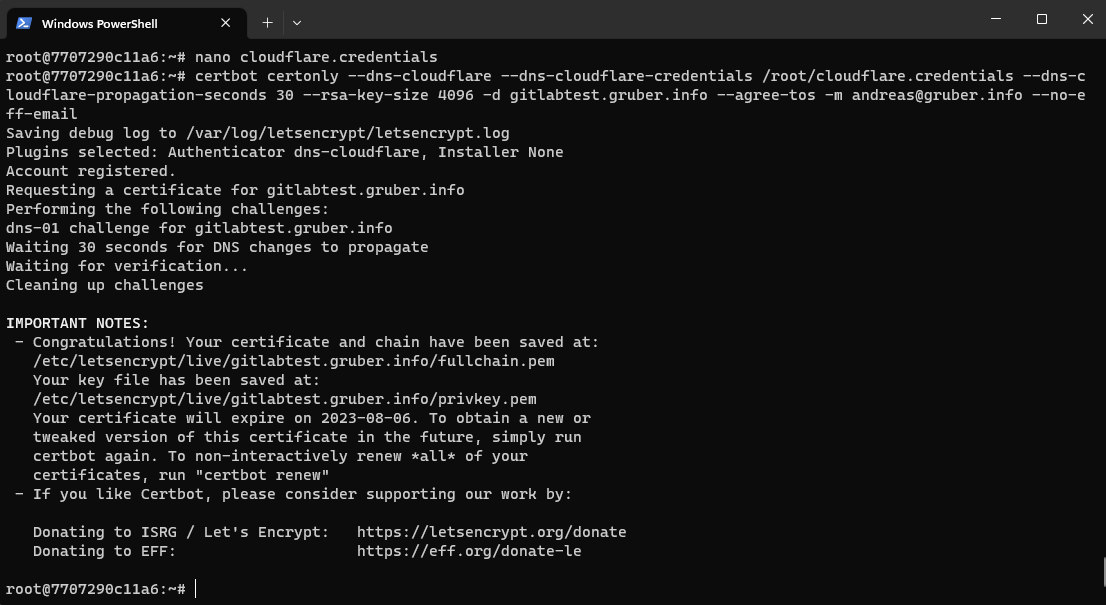
\includegraphics[width=14cm]{images/lets_encrypt.png}
	\caption{Let´s encrypt DNS-01 challenge}
	\label{fig:lets_encrypt}
\end{figure}

In the 'gitlabrunners' network a fixed IP of '10.0.0.99' is set for this machine, which can be used by the Runners to access GitLab.\\

\subsection{OS configuration}

Login to the OS is only possible via SSH and SSH keys. Login with password is not possible. 

As the 2GByte of memory is still not enough, a swap-file of 6GByte in size is added to the system (\ref{fig:swapfile}).
Without this, GitLab would not be able to start.

\begin{figure}[H]
	\centering
	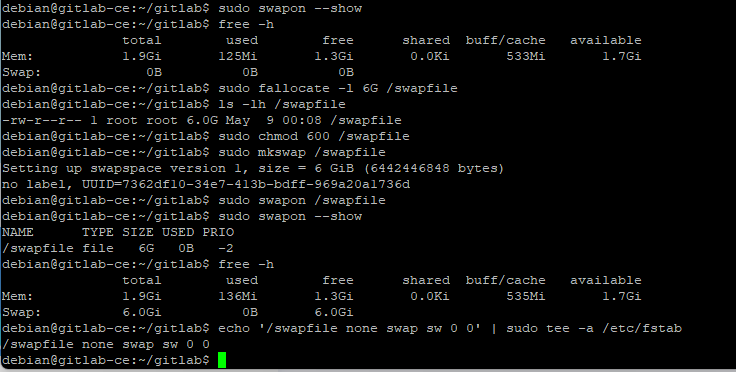
\includegraphics[width=14cm]{images/swapfile.png}
	\caption{Adding a swapfile}
	\label{fig:swapfile}
\end{figure}

Docker is installed according to the official Docker documentation (\cite{refDockerDebian}).
